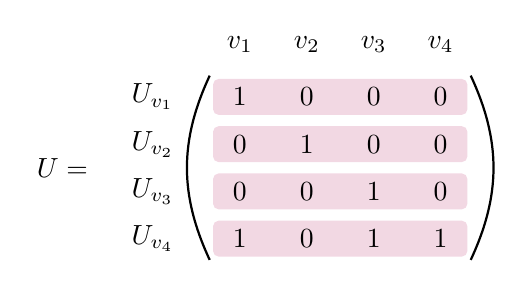
\begin{tikzpicture}[baseline=(current bounding box.center), x=0.85cm, y=0.6cm]
  % U = matriz de vecindades mínimas (vacía): columnas v_k, filas U_{v_k}
  \definecolor{RosaPoster}{RGB}{205,100,145}% rosa de los resaltados del póster
  % Resaltado de la fila que se está calculando
  % {fila resaltada/diapositiva}
  \foreach \fil/\dia in {1/2, 2/3, 3/4, 4/5}
    \fill<\dia>[RosaPoster, opacity=0.25, rounded corners=2pt] (0.6,-\fil-0.38) rectangle (4.4,-\fil+0.38);
  \node at (-1.65,-2.5) {$U=$};
  % Etiquetas de filas y columnas
  \foreach \k in {1,...,4} {
    \node at (\k,0.1) {$v_{\k}$};
    \node at (-0.3,-\k) {$U_{v_{\k}}$};
  }
  % Paréntesis
  \draw[thick] (0.55,-0.55) to[bend right=25] (0.55,-4.45);
  \draw[thick] (4.45,-0.55) to[bend left=25] (4.45,-4.45);
  % Entradas: {fila/columna/valor/diapositiva de aparición}
  \foreach \fil/\col/\val/\dia in {1/1/1/2, 1/2/0/2, 1/3/0/2, 1/4/0/2,
                                   2/1/0/3, 2/2/1/3, 2/3/0/3, 2/4/0/3,
                                   3/1/0/4, 3/2/0/4, 3/3/1/4, 3/4/0/4,
                                   4/1/1/5, 4/2/0/5, 4/3/1/5, 4/4/1/5}
    \node<\dia-> at (\col,-\fil) {$\val$};
\end{tikzpicture}
